% Anhang ist manuell erstellt und verwendet nicht das appendix package
\setcounter{section}{0}
\setcounter{subsection}{0}
\renewcommand*\thesection{\Alph{section}}

\chapter{Anhang}
\section{Navigationsstruktur}

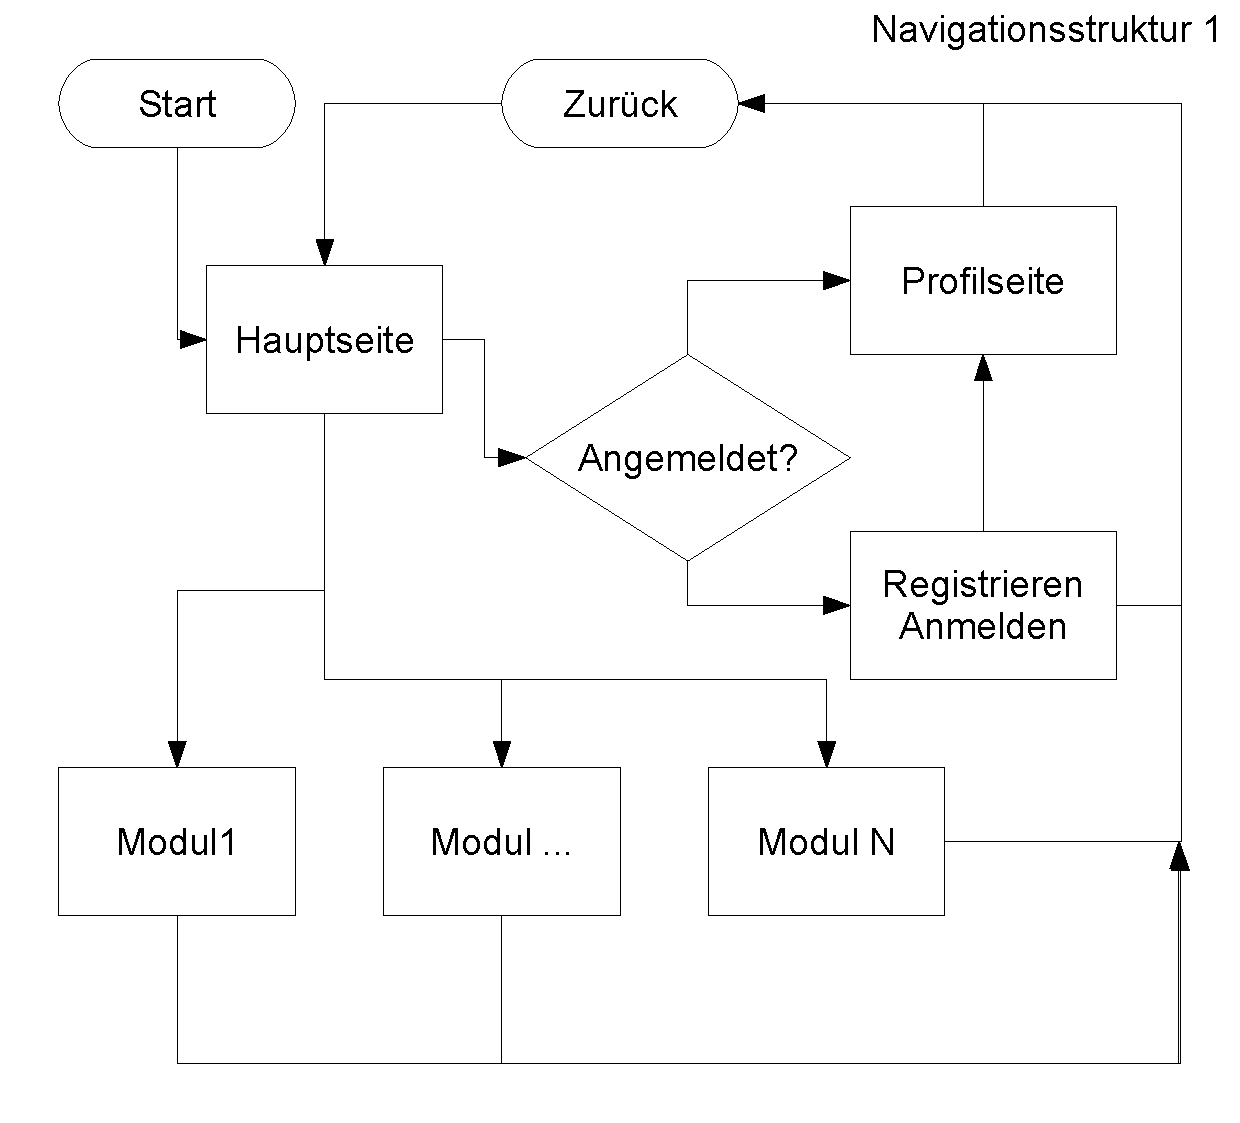
\includepdf[pages={1-2}]{navigation.pdf}

\section{Layout}

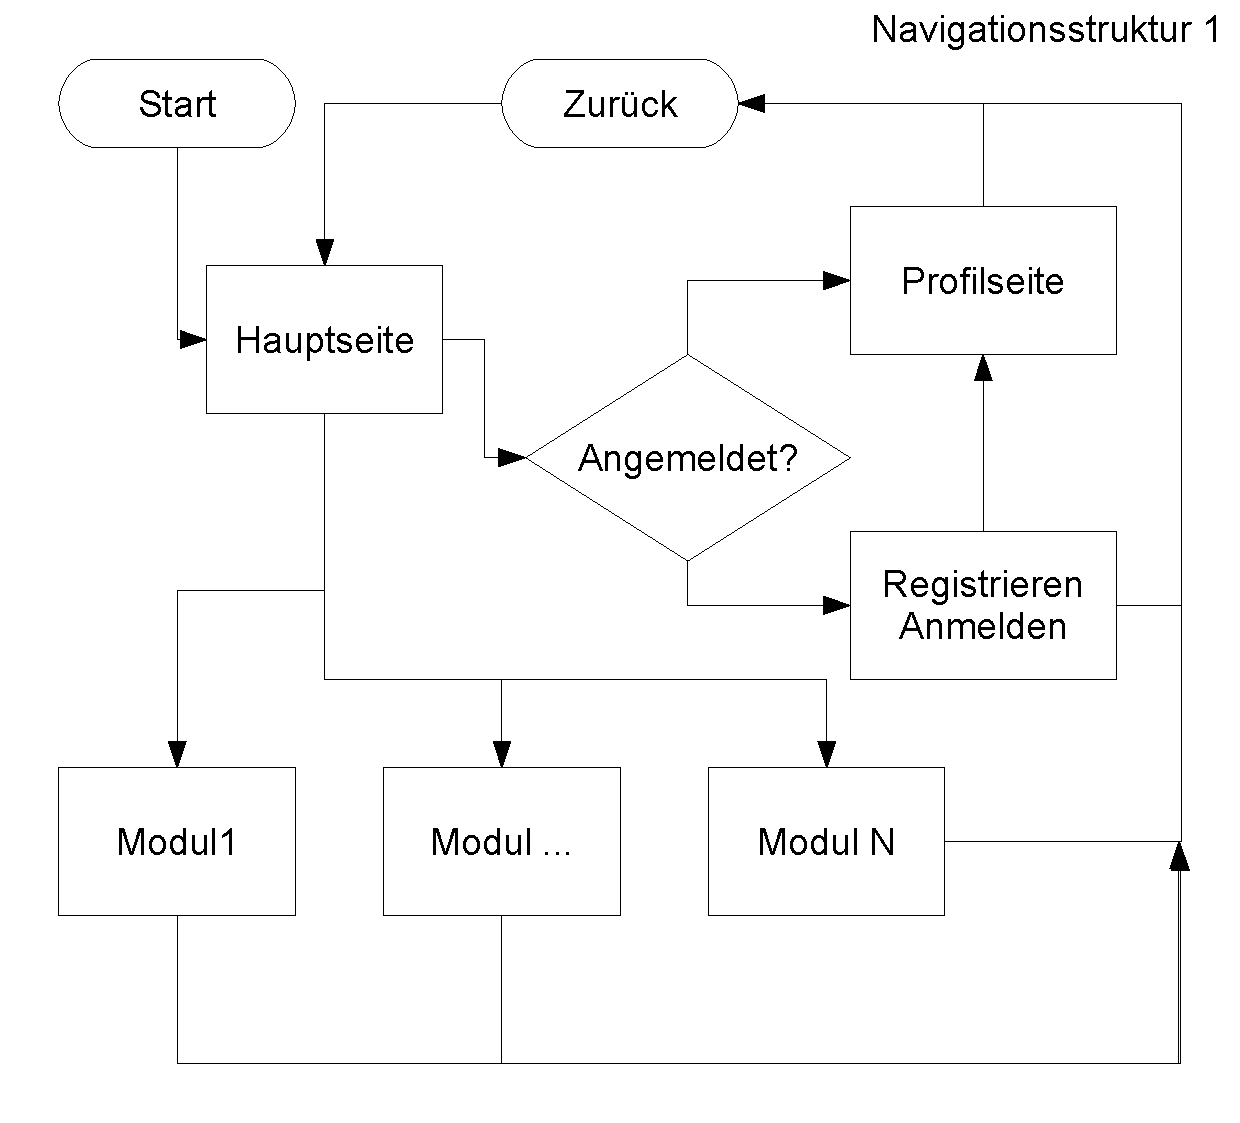
\includepdf[pages={1-7}]{struktur.pdf}


\section{Modul Mathematik}
\subsection{Texte}
\begin{tabular}{ | l | l | } 
  \texttt{mathematics/index.html        } & Hauptseite. Intro Vedische Mathematik \\
  \texttt{mathematics/learn/index.html  } & Lern- Hauptseite. Vorstellung der Inhalte, \\
  \texttt{mathematics/learn/page1.html  } & Alle von 9, den letzten von 10 \\
  \texttt{mathematics/learn/page2.html  } & Vertikal und Kreuzweise \\
  \texttt{mathematics/learn/page2a.html } & Vertikal und Kreuzweise Für kleine Zahlen \\
  \texttt{mathematics/learn/page2b.html } & Vertikal und Kreuzweise Für Zahlen nahe 100 \\
  \texttt{mathematics/learn/page2c.html } & Vertikal und Kreuzweise Für Zahlen unter 100 \\
  \texttt{mathematics/learn/page2d.html } & Vertikal und Kreuzweise Für kleine Brüche \\
  \texttt{mathematics/learn/page3.html  } & Um 1 mehr als bei dem davor \\
  \texttt{mathematics/learn/page4.html  } & Multiplikation mit 11 \\
  \texttt{mathematics/learn/page5.html  } & Division durch 9 \\
  \texttt{mathematics/learn/index.html  } & Trainings- Hauptseite. \\
  \texttt{mathematics/learn/page1.html  } & Vertikal und Kreuzweise \\
  %\texttt{mathematics/learn/page2.html  } & \\
  \texttt{mathematics/learn/page2a.html } & Vertikal und Kreuzweise Für kleine Zahlen \\
  \texttt{mathematics/learn/page2b.html } & Vertikal und Kreuzweise Für Zahlen nahe 100 \\
  \texttt{mathematics/learn/page2c.html } & Vertikal und Kreuzweise Für Zahlen unter 100 \\
  \texttt{mathematics/learn/page2d.html } & Vertikal und Kreuzweise Für kleine Brüche \\
  \texttt{mathematics/learn/page3.html  } & Um 1 mehr als bei dem davor \\
  \texttt{mathematics/learn/page4.html  } & Multiplikation mit 11 \\
  \texttt{mathematics/learn/page5.html  } & Division durch 9 \\
\end{tabular}

\subsection{Layout}
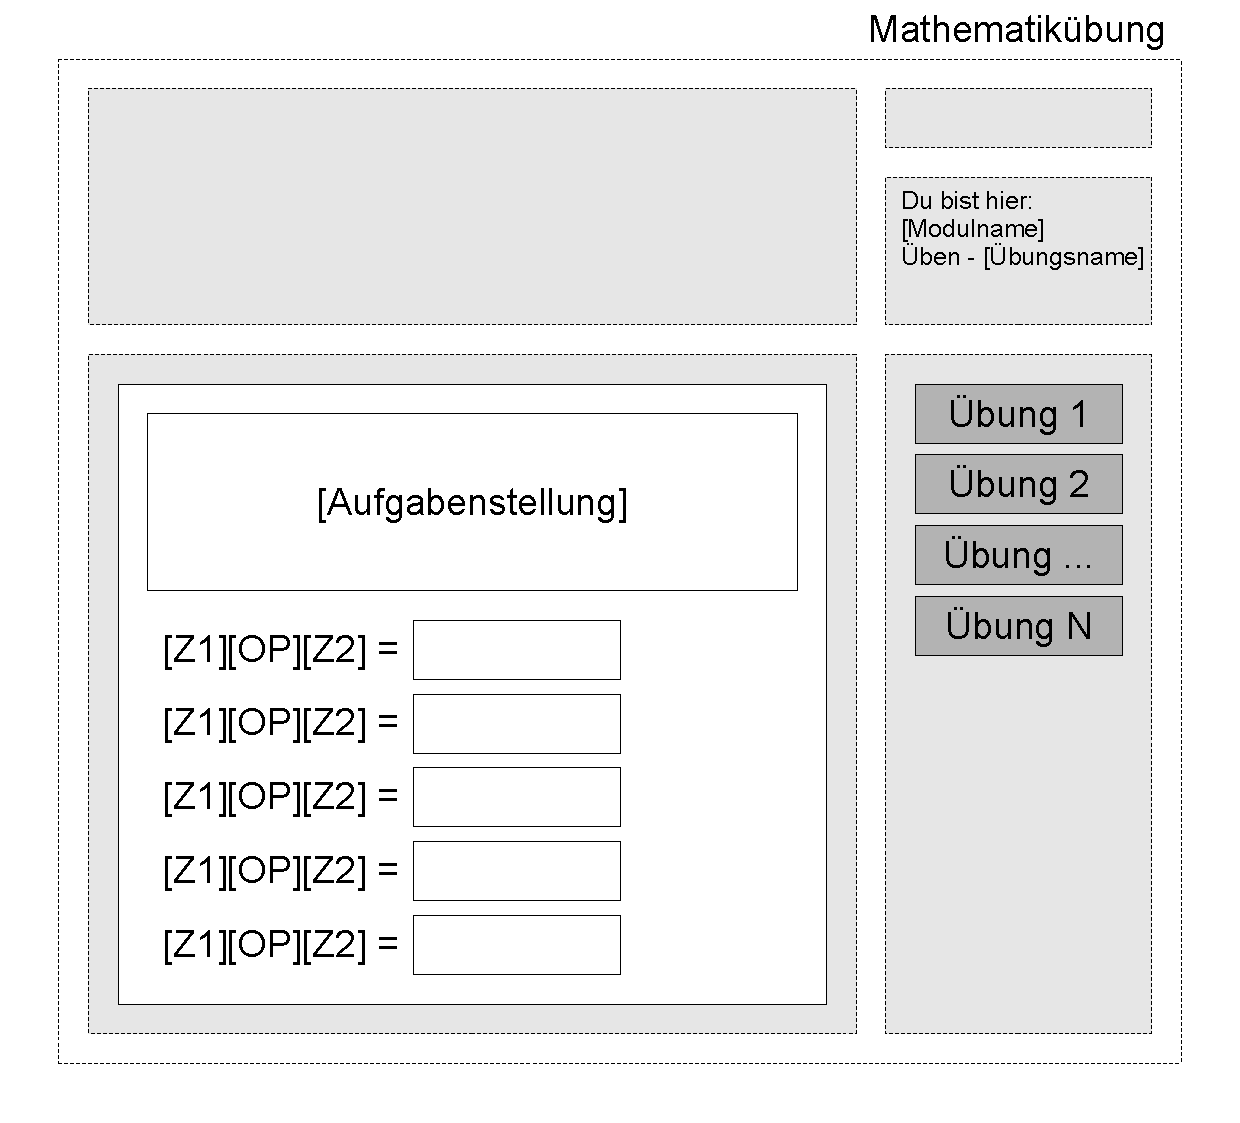
\includepdf[pages={1}]{math-practise-page.pdf}